% !TEX TS-program = pdflatex
% !TEX root = ../main.tex

\chapter{Figures and Tables}
\label{ch:figures_tables}
In this chapter we will see some examples of tables and figures.

\section{Figures}
Let's see now how to put one or several images in your text.


\begin{figure}[ht]
    \centering
    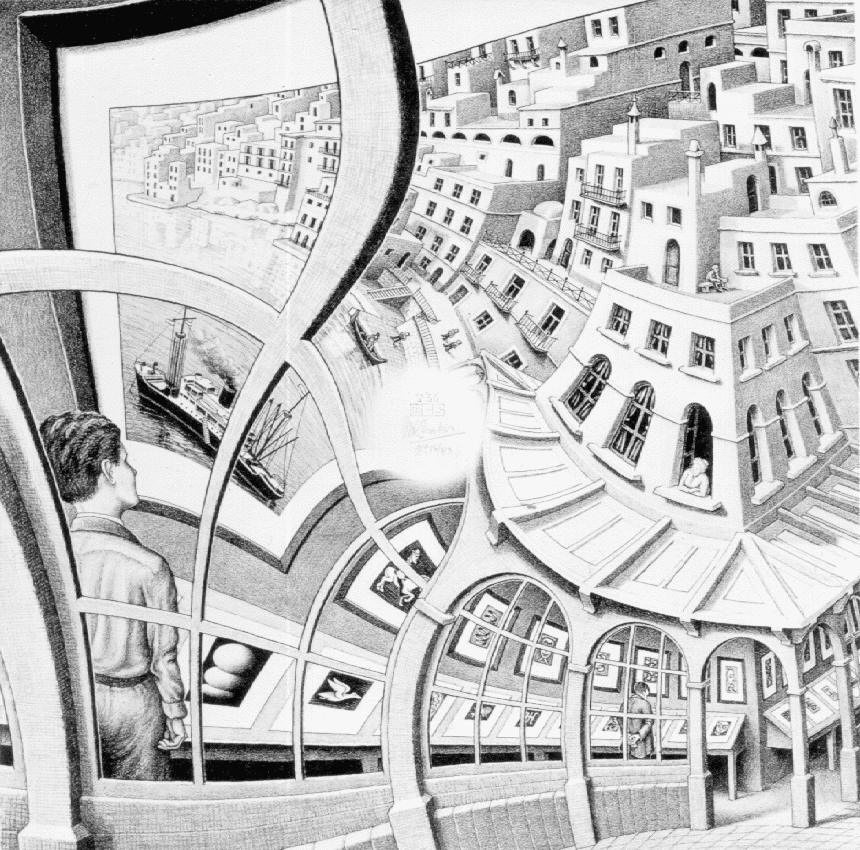
\includegraphics[width=0.5\columnwidth]{../figures/images/galleria_stampe}
    \caption[A floating figure]{A floating figure (the lithograph \emph{Galleria di stampe}, of M.~Escher, got from \url{http://www.mcescher.com/}).}
    \label{fig:galleria}
\end{figure}

\begin{figure}[tb]
    \centering
    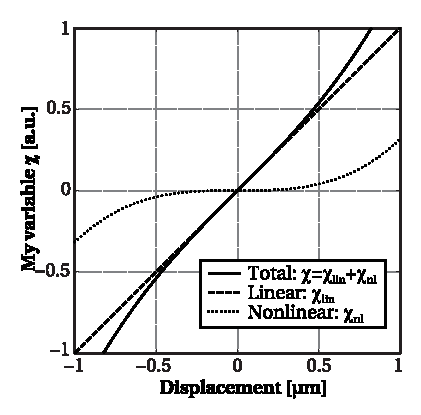
\includegraphics{../figures/images/some_vector_graphics}
    \caption[A floating figure]{A floating figure with text typeset in "Utopia Latex", a font provided in the template-folder for typesetting figures with greek characters. The text has been "outlined" for best compatibility with the repro during the printing.}
    \label{fig:vector_graphics}
\end{figure}

The figure~\ref{fig:galleria} is a floating figure and was obtained with the following code:
\begin{lstlisting}
\begin{figure}[tb] 
\centering 
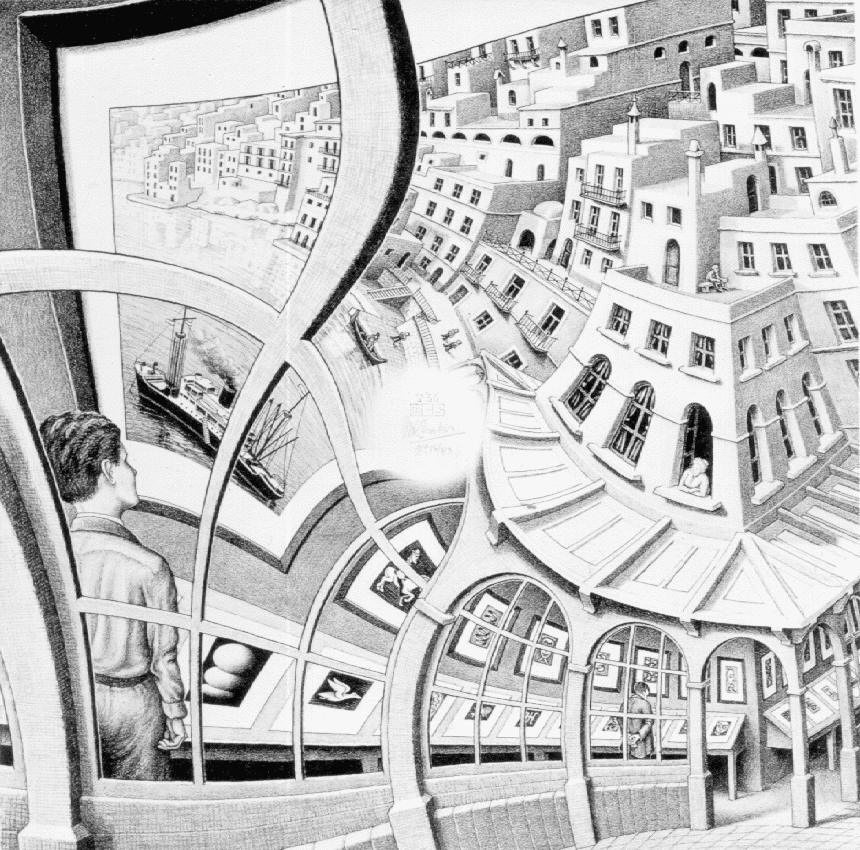
\includegraphics[width=0.5\columnwidth]{../figures/images/galleria_stampe} 
\caption[A floating figure]{A floating figure ... }
\label{fig:galleria} 
\end{figure}
\end{lstlisting}


\lipsum[1-2]

\begin{figure}[tb]
    \centering

    \subfloat[Asia personas duo.]
    {\includegraphics[width=.45\columnwidth]{../figures/images/lorem}} \quad
    \subfloat[Pan ma signo.]
    {\label{fig:ipsum}%
        
\includegraphics[width=.45\columnwidth]{../figures/images/ipsum}} \\
    \subfloat[Methodicamente o uno.]
    {
\includegraphics[width=.45\columnwidth]{../figures/images/dolor}} \quad
    \subfloat[Titulo debitas.]
    {
\includegraphics[width=.45\columnwidth]{../figures/images/sit}}
    \caption[Tu duo titulo debitas latente]{Tu duo titulo debitas
        latente.}
    \label{fig:example}
\end{figure}

The figure~\ref{fig:example} is a floating figure and was obtained with the following code:
\begin{lstlisting}
\begin{figure}[tb]
\centering
\subfloat[Asia personas duo.]
{\includegraphics[width=.45\columnwidth]{lorem}} \quad
\subfloat[Pan ma signo.]
{\label{fig:ipsum}%

\includegraphics[width=.45\columnwidth]{ipsum}} \\
\subfloat[Methodicamente o uno.]
{
\includegraphics[width=.45\columnwidth]{dolor}} \quad
\subfloat[Titulo debitas.]
{
\includegraphics[width=.45\columnwidth]{sit}}
\caption[Tu duo titulo debitas latente]{Tu duo titulo debitas latente.}
\label{fig:example}
\end{figure}
\end{lstlisting}

\begin{figure}[t]
    \centering
    \resizebox{.45\textwidth}{!}{\subimport{../figures/}{block_diagram}}
    \label{fig:control_diagram}
    \caption{Control Structure.}
\end{figure}

\lipsum[3-8]

\section{Tables}
Let's see how to make a well designed table.

\begin{table}[tb]
    \caption[A floating table]{A floating table.}
    \label{tab:example}
    \centering
    \begin{tabular}{ccc}
        \toprule
        name  & weight & food   \\
        \midrule
        mouse & 10 g   & cheese \\
        cat   & 1 kg   & mice   \\
        dog   & 10 kg  & cats   \\
        t-rex & 10 Mg  & dogs   \\
        \bottomrule
    \end{tabular}
\end{table}

The table~\ref{tab:example} is a floating table and was obtained with the following code:
\begin{lstlisting}
\begin{table}[tb]
\caption[A floating table]{A floating table.}
\label{tab:example}
\centering
\begin{tabular}{ccc}
\toprule
	name 	& weight & food	  \\ 
\midrule
	mouse	& 10  g	 & cheese \\
	cat		&  1 kg	 & mice	  \\
	dog		& 10 kg	 & cats   \\
	t-rex	& 10 Mg	 & dogs	  \\
\bottomrule 
\end{tabular}
\end{table}
\end{lstlisting}

\lipsum[1-2]

\begin{table}[t]
    \centering
    \resizebox{\textwidth}{!}{\subimport*{../tables}{table_results}}
    \vspace{2mm}
    \caption{Some other more elaborated table.}
    \label{tab:hd_results}
\end{table}